\documentclass[UTF8, a4paper, 11pt]{article}
\usepackage{diagbox}
\usepackage{subfigure}
\usepackage[UTF8, scheme=plain]{ctex}
\usepackage{fontspec}
\usepackage{float}
\usepackage{amsmath}
\newtheorem{myDef}{Definition}
\usepackage{graphicx}
\usepackage{geometry}
\usepackage{listings}
\usepackage{xcolor}
\usepackage{caption}
\geometry{scale=0.8}
\linespread{1.5}
\usepackage{hyperref}
\usepackage{color}
\usepackage{fontspec}
\usepackage{enumitem}
\usepackage[linesnumbered,boxed]{algorithm2e}    
\usepackage{xeCJK}
\usepackage{indentfirst} 
\graphicspath{{Pics/}} 	% 在于.tex同级的目录下创建名为pic的文件夹,存放图片


\setlength{\parindent}{2em}

\lstset{
    language={python},
    frame=shadowbox,
    breaklines=true,
    numbers=left,
    backgroundcolor=\color[RGB]{245,245,244},
    rulesepcolor=\color{red!20!green!20!blue!20},
    numberstyle={\color[RGB]{0,192,192}\tiny},
    basicstyle=\footnotesize \fontspec{Source Code Pro}
}
\setenumerate[1]{itemsep=0pt,partopsep=0pt,parsep=\parskip,topsep=0pt}
\setitemize[1]{itemsep=0pt,partopsep=0pt,parsep=\parskip,topsep=0pt}
\setdescription{itemsep=0pt,partopsep=0pt,parsep=\parskip,topsep=0pt}


\title{	
\normalfont \normalsize
\textsc{School of Data and Computer Science, Sun Yat-sen University} \\ [25pt] %textsc small capital letters
\rule{\textwidth}{0.5pt} \\[0.4cm] % Thin top horizontal rule
\huge 作业1\\ % The assignment title
\rule{\textwidth}{2pt} \\[0.5cm] % Thick bottom horizontal rule
\author{18308045 谷正阳}
\date{\normalsize\today}
}

\begin{document}
\maketitle
\tableofcontents
\newpage
\section{文件组织}
\begin{itemize}
    \item test\_a:一维VS二维,计算EPOCHS轮,取平均时间当作效率,矩阵大小1024x1024
    \item test\_b:线程块大小对性能的影响,计算EPOCHS轮,取平均时间当作效率,矩阵大小1024x1024
    \item test\_c:每个线程计算的元素数量对性能的影响,计算EPOCHS轮,取平均时间当作效率,矩阵大小1024x1024
    \item test\_d:以上配置在处理不同大小的矩阵时,性能可能的差异
    \begin{itemize}
        \item 1000\_1000:矩阵大小1000x1000
        \begin{itemize}
            \item test\_a
            \item test\_b
            \item test\_c
        \end{itemize}
        \item 8192\_8192:矩阵大小8192x8192
        \begin{itemize}
            \item test\_a
            \item test\_b
            \item test\_c
        \end{itemize}
    \end{itemize}
    \item hw1.h:CUDA实现用到的函数,函数已写注释
    \item openmp.cpp:OpenMp实现,一维数组表示矩阵,4线程,每个线程对数组中相邻数据做运算。计算EPOCHS轮,取平均时间当作效率,在大小为1000x1000,1024x1024,8192x8192的矩阵上分别讨论效率
\end{itemize}
\section{CUDA实现}
实现细节见hw1.h的代码及注释。
\subsection{一维VS二维}
\begin{figure}[H]
    \centering
    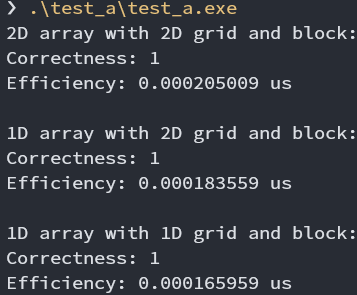
\includegraphics[width=0.4\textwidth]{test_a.png}
\end{figure}
一维数组,grid,block效率最高。原因是二维数组A[y][x]内存访问次数多于A[y * m + x],效率低;二维grid,block使用一维数组,同一个block内线程空间不连续,效率低。
\subsection{线程块大小对性能的影响}
\begin{figure}[H]
    \centering
    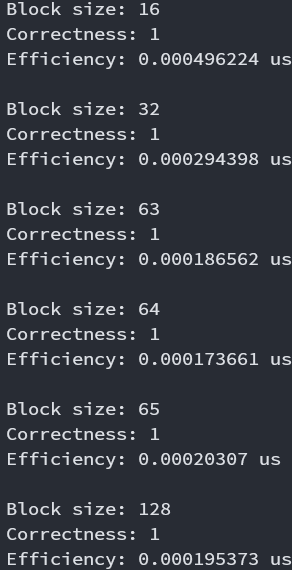
\includegraphics[width=0.4\textwidth]{test_b.png}
\end{figure}
16、32效果差,64、128效果接近,block size是否是32整数倍影响不是很大(有时128、63、65用时比64少)。block size最好32整数倍的原因是,一个SM执行一个block中的所有线程,而SM负责执行和调度warp即以32个线程为一个单位,因而要最大化利用warp,block size需要是32的整数倍。
\subsection{每个线程计算的元素数量对性能的影响}
\begin{figure}[H]
    \centering
    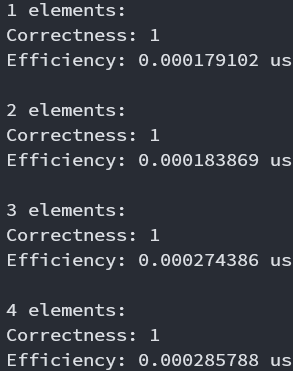
\includegraphics[width=0.4\textwidth]{test_c.png}
\end{figure}
元素数量越多,性能越差。因为处理多个元素时是串行的,而且运用了循环结构,GPU不太适用于复杂控制流。
\subsection{以上配置在处理不同大小的矩阵时}
\subsubsection{1000x1000}
\begin{figure}[H]
    \centering
    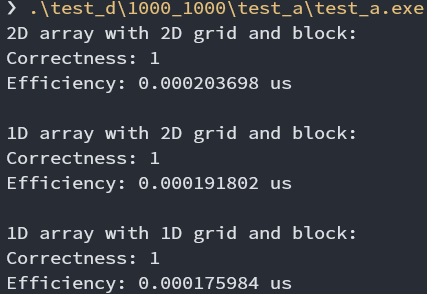
\includegraphics[width=0.4\textwidth]{1000_a.png}
\end{figure}
\begin{figure}[H]
    \centering
    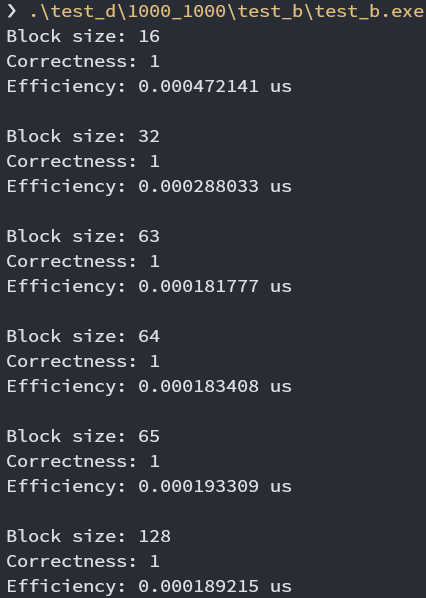
\includegraphics[width=0.4\textwidth]{1000_b.png}
\end{figure}
\begin{figure}[H]
    \centering
    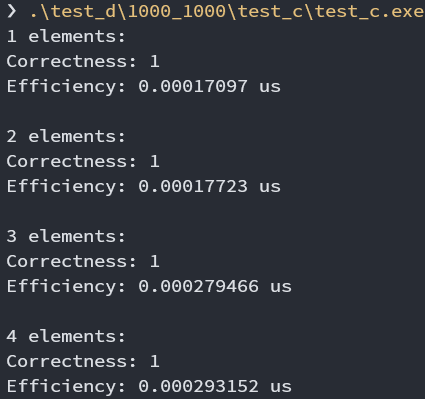
\includegraphics[width=0.4\textwidth]{1000_c.png}
\end{figure}
矩阵变小时,上述结论基本没有变化。
\subsubsection{8192x8192}
\begin{figure}[H]
    \centering
    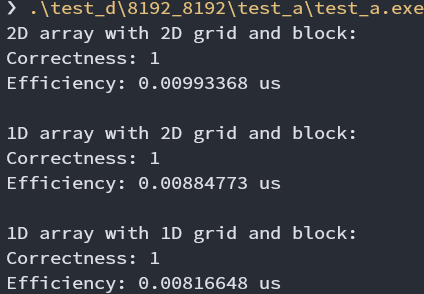
\includegraphics[width=0.4\textwidth]{8192_a.png}
\end{figure}
\begin{figure}[H]
    \centering
    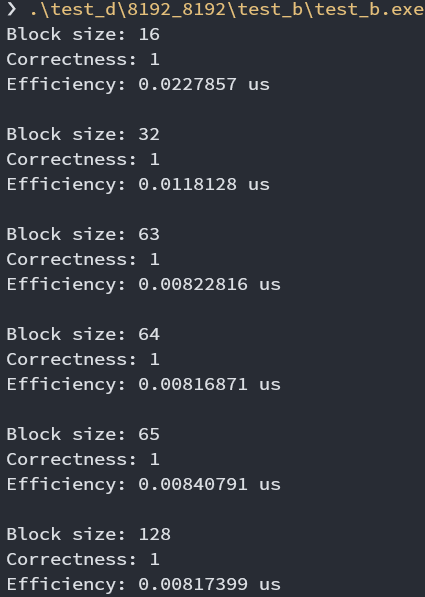
\includegraphics[width=0.4\textwidth]{8192_b.png}
\end{figure}
\begin{figure}[H]
    \centering
    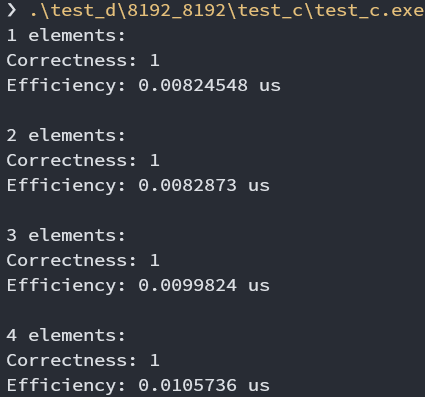
\includegraphics[width=0.4\textwidth]{8192_c.png}
\end{figure}
矩阵变大时,上述结论基本没有变化。
\section{OpenMp实现}
\begin{figure}[H]
    \centering
    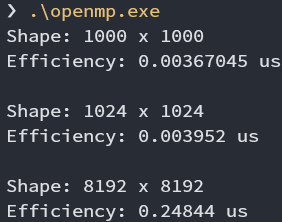
\includegraphics[width=0.4\textwidth]{openmp.png}
\end{figure}
都比CUDA实现效率低,对于更大的矩阵效率更低,原因是线程数远少于CUDA实现,矩阵越大并行程度越低。
%\clearpage
%\bibliography{E:/Papers/LiuLab}
%\bibliographystyle{apalike}
\end{document}
%%% Local Variables:
%%% mode: latex
%%% TeX-master: t
%%% End:
